\documentclass[a4paper, 11pt]{tubsreprt}
\usepackage[ngerman]{babel}
\usepackage[utf8]{inputenc}
\usepackage{cite}
\usepackage{graphicx}
\usepackage{wrapfig}
\title{Wärmebehandlung}
\date{Wintersemester 17/18}
\author{J. Hansen, S. Vodde,
 J. Veer, T. Stein}

\logo{
	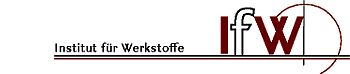
\includegraphics{Bilder/ifw-logo.jpg}
}

\begin{document}
\maketitle
\tableofcontents
\chapter{Titanwerkstoffe}
\section{Gefügemerkmale}
Wie andere Metalle liegt Titan in verschiedenen Gefügezuständen beziehungsweise Phasenzuständen vor. Der Zustand ist von der Temperatur und den vorliegenden Legierungselementen abhängig. Bei reinem Titan liegt unterhalb von 882°C Grad ein hexagonal dichtest gepackte Kristallstruktur vor. Diese Phase wird als Alphaphase ($\alpha$-Phase) bezeichnet. Oberhalb von 882°C liegt die Kristallstruktur in einer kubisch raumzentrierten Anordnung vor ($\beta$-Phase). Die Umwandlungstemperatur ist für jede Titanlegierung unterschiedlich und ist von den Legierungselementen abhängig. Sie wird als Betatransustemperatur bezeichnet \cite{Luetjering2007}.



\subsection{Alpha}
Die alpha-Titan Phase ist durch eine hexagonale Gitterstruktur gekennzeichnet. Dadurch entsteht ein anisotropes Werkstoffverhalten in einem Einkristall.
Ein Einkristall ist über ein homogenes, einhaltliches Kristallgitter definiert.
In einem Belastungsfall dieses Einkristalls ist das Werkstoffverhalten abhängig von der Belastungsrichtung, im Verhältnis zur Gitterrichtung. Das Elastizitätsmodul $E$ reicht je nach Verhältnis, von minimal 100 GPa bis maximal 145 GPa. Es ist eine Kenngröße, die das elastische Verhalten eines Werkstoffes definiert und wird in Pascal angegeben. 

Titan wird jedoch sehr selten als Einkristall hergestellt, sodass die unterschiedliche Kornorientierung dafür sorgt, das die anisotropie der einzelnen Körner sich gegenseitig aufhebt. Man kann somit von einem isotropen Werkstoffverhalten ausgehen.

\subsection{Beta}
Eine $\beta$-Phase ist ein Gefüge mit einer kubisch raumzentrierte Gitteranordnung. Dadurch resultiert ein homogenes Werkstoffverhalten.

Das E-Modul und die Festigkeit der Betaphase ist deutlich geringer als die Alphaphase. Das E-Modul der Betaphase erreicht

Eine große menge an $\beta$-Phase existiert in der Regel bei Raumtemperatur nur unter bestimmten Bedingungen. Sie kann als metastabile Phase auftreten. Dies bedeutet, dass das Material nicht vollständig den Phasenübergang abschließen konnte und so in dem Zustand aus höheren Temperaturen verblieben ist. 

Durch Zusatz bestimmter Legierungselemente kann sie auch in größeren Mengen vorliegen. Dies wird im Kapitel Betastabilisierende Legierungselemente näher erläutert.
\subsection{Gefüge}
Da sich die Arbeit vor allem mit Gefügeausprägungen und ihren Auswirkungen auseinandersetzt, werden die grundlegenden hier vorgestellt. Die jeweiligen Ausprägungen sind Ausschlaggebend wie sich das Material mechanisch verhält. Da die mögliche Wärmebehandlung nach dem Rekristallisieren statt findet, sind einige Gefügeausbildungen möglicherweise nicht möglich. Dies ist abhängig von dem Ausgangsgefüge.
Es sind auch Kombinationen der einzelnen Gefüge möglich, um Vorteile der einzelnen hinsichtlich ihrer mechanischen Eigenschaften zu kombinieren.
\subsubsection{Lamellar}
In Abbildung 1.1 ist ein Volllamellares Gefüge zu sehen. Es Kennzeichnet sich durch fein parallel verlaufende Nadeln. Die breite der einzelnen Nadeln hängt mit der Abkühlgeschwindigkeit zusammen. In dieser Abbildung wurde eine schnelle Abkühlung gewählt, was zu kleinen, feinen Nadeln führt. 

Lamallare Gefüge entstehen aus einer Abkühlung aus dem $\beta$-Gebiet. Während des Abkühlens bilden sich in den Korngrenzen der $\beta$-Phase $\alpha$-Bereiche die in das $\beta$-Korn hinein wachsen. Die Alphabereiche wachsen erst in eine Richtung bevor sie ihre Dicke erhöhen. 

\begin{minipage}{\textwidth}


	\centering
		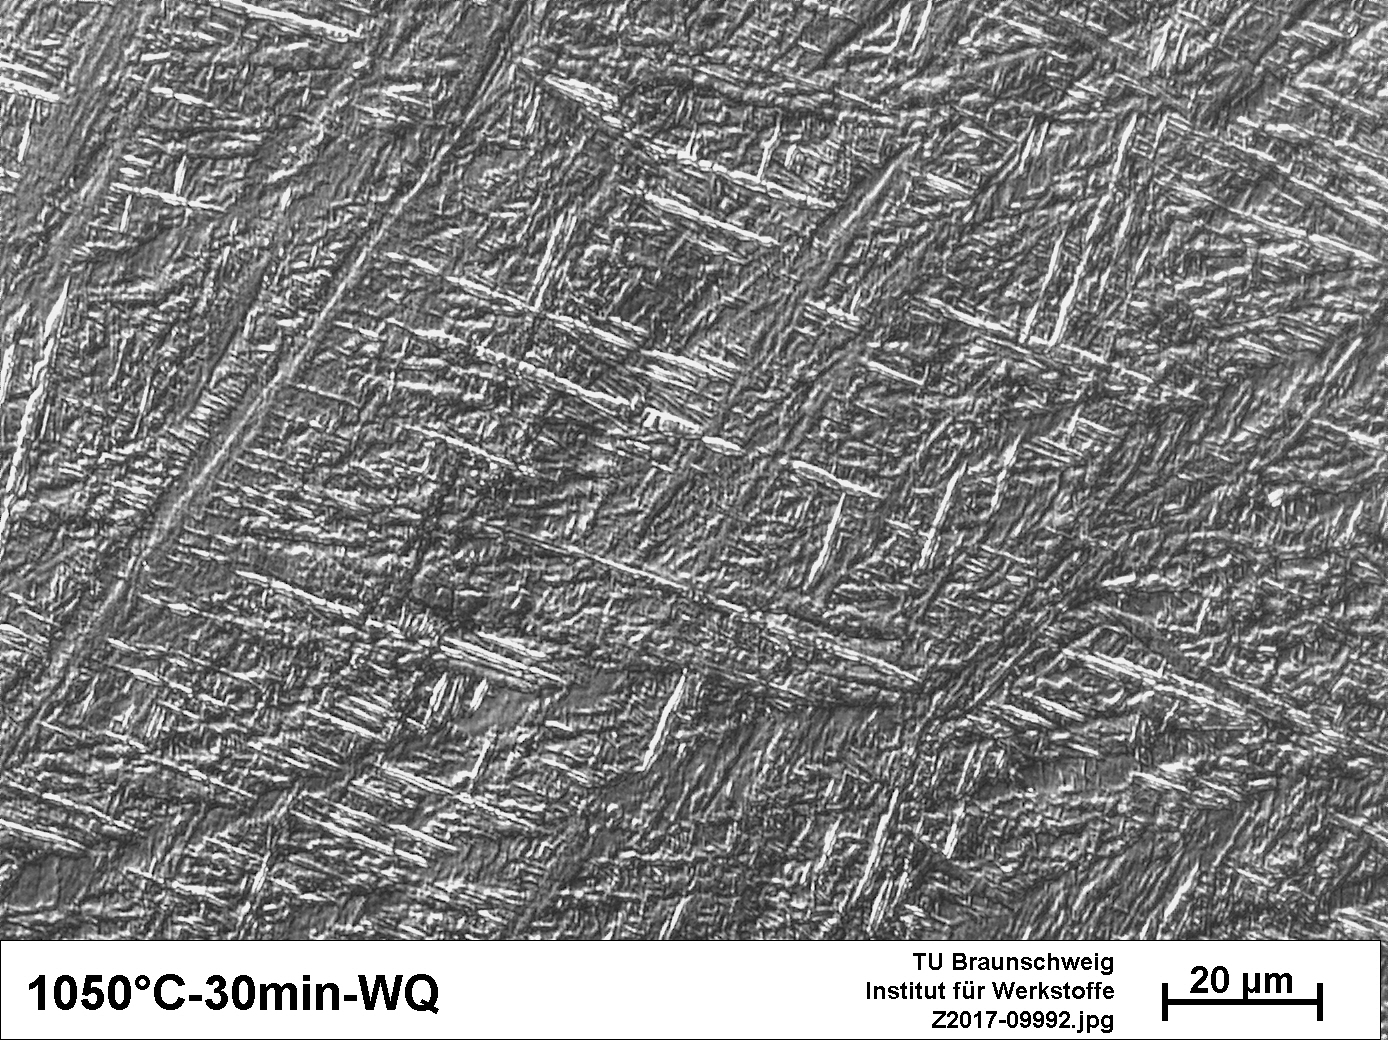
\includegraphics[scale=0.5]{Bilder/Vollmartensit.jpg}
		\captionof{figure}{Volllamellares Gefüge}
		\label{fig1}
		
\end{minipage}


\subsubsection{Bimodal}
\subsubsection{Globular}
\chapter{Methodik}
\section{Wärmebehandlung}

Die Wärmebehandlung nach der Rekristllisation ist die letzte Methode um das Gefüge des Titans einzustellen. Hierbei kommt es auf Parameter wie Temperatur, Haltezeit und Abkühlmethode an. Um die bereits erwähnten Gefüge zu realisieren, ist eine spezifische Abfolge von einer beziehungsweise mehreren Stufen einer Wärmebehandlung nötig. Die grundlegenden Behandlungen werden in diesem Kapitel behandelt. Spezielle, mehrstufige Behandlungen werden in dem dritten Kapitel behandelt.
\paragraph{Temperaturkontrolle}
Für die Temperaturkontrolle innerhalb der Wärmebehandlung kommt ein Ofen zum Einsatz. Dieser kann bis Temperaturen weit über Betatransus aufheizen und diese, mit einer Genauigkeit von drei Kelvin, halten. 

Der Ofen ist außerdem für die Aufheizgeschwindigkeit verantwortlich, da diese auch einen wichtigen Einfluss haben kann.
\paragraph{Abkühlmedien}

\subsection*{Anpassung der Gefüge durch Wärmebehandlung}
\bibliographystyle{plain}
\bibliography{literatur}

\end{document}
